\section{Database Annotation Errors} \label{sec:Clustering_Anomalies}

To evaluate the anomalies in \autoref{fig:PCA_Cluster_Knee_4} \textbf{\textsf{B}} and \textbf{\textsf{C}}, an evolutionary distance was calculated by \gls{MSA} for every eventually misplaced sequence (\autoref{sec:MAFFT}). Therefore, the eventually misplaced sequence was compared to a sample of five sequences from the same cluster related to the dominant subtype of the cluster, as well as to a sample of five sequences with subtype equal to the misplaced sequence but from other clusters. The mean of distances was then calculated for both cases to rate the assignment and reveal possible misannotations in the \gls{IRD}. 

\begin{table}[!hbt]
    \centering
    \caption[Anomalies in Segment 4 Cluster 2 (\texttt{PCA})]{\textbf{Anomalies in Segment 4 Cluster 2 (\texttt{PCA}).} The \glspl{MSA} mean distance of the given sequences in comparison to a sample of H1 sequences of the same cluster and a sample of H10 sequences present in other clusters.}
    \label{tab:PCA_Error_4_2}
    \pgfplotstabletypeset[
        every head row/.style={
            before row={
                \toprule
            },
            after row={
                \midrule
            },
        },
        every last row/.style={
            after row={
                %... & ... & ... & ... & ... & ... & ... & ...\\
                \bottomrule
            },
        },
        begin table=\begin{tabular*}{0.75\textwidth},
        end table=\end{tabular*},
        columns={0,1,2},
        columns/0/.style={string type,multicolumn names=l,column name=\textbf{Accession}, column type=@{\extracolsep{\fill}\hspace{6pt}}l},
        columns/1/.style={multicolumn names=l,column name=\textbf{H1}, column type=l},
        columns/2/.style={multicolumn names=l,column name=\textbf{H10}, column type=l},
    ]
    {PCA/error_segment_4_cluster_2_difference_head.csv}
\end{table}

In case of \autoref{fig:PCA_Cluster_Knee_4} \textbf{\textsf{C}}, a single sequence with subtype H10 was classified as belonging to cluster 2 which other than that completely consists of H1 and unclassified sequences. By investigation on this possible misplacement the mentioned comparison with \gls{MSA} was used. The results for this comparison in \autoref{tab:PCA_Error_4_2} points to the fact, that the as H10 annotated sequence with accession MK237334 is related to subtype H1. The mean of evolutionary distance based on \glspl{MSA} is very low in comparison to a sample of cluster 0 H1 sequences especially when considering the size of cluster 0. The distance in comparison to a sample of random H10 sequences is much higher. 

When considering the random sampling on the different H10 clusters and the possible error by high differences between the sequences of the clusters, a misannotation is still more likely. Furthermore, only this sole sequence, annotated as subtype H10, is present in a cluster of over 900 sequences of H1 with a very low distance to the H1 sequence sample of the same cluster. 

\begin{table}[!hbt]
    \centering
    \caption[Anomalies in Segment 4 Cluster 48 (\texttt{PCA})]{\textbf{Anomalies in Segment 4 Cluster 48 (\texttt{PCA}).} The \glspl{MSA} mean distance of the given sequences in comparison to a sample of H16 sequences of the same cluster and a sample of H13 sequences present in another cluster. Only the first 20 columns are presented here, the full table can be found in the \href{https://github.com/ahenoch/Masterthesis.git}{Projects GitHub Repository}.}
    \label{tab:PCA_Error_4_48}
    \pgfplotstabletypeset[
        every head row/.style={
            before row={
                \toprule
            },
            after row={
                \midrule
            },
        },
        every last row/.style={
            after row={
                ... & ... & ...\\
                \bottomrule
            },
        },
        begin table=\begin{tabular*}{0.75\textwidth},
        end table=\end{tabular*},
        columns={0,1,2},
        columns/0/.style={string type,multicolumn names=l,column name=\textbf{Accession}, column type=@{\extracolsep{\fill}\hspace{6pt}}l},
        columns/1/.style={multicolumn names=l,column name=\textbf{H16}, column type=l},
        columns/2/.style={multicolumn names=l,column name=\textbf{H13}, column type=l},
    ]
    {PCA/error_segment_4_cluster_48_difference_head.csv}
\end{table}

When comparing the distances for \autoref{fig:PCA_Cluster_Knee_4} \textbf{\textsf{C}} in \autoref{tab:PCA_Error_4_48}, no decision for misannotation can be made. The dominant subtype in the cluster 48 is H16 but the sequences of subtype H13 that seem to be misplaced in the cluster have a smaller distance to the sample of sequences from subtype H13. The difference in distance to sample sequences of H13 as well as for sequences for H16 gave indeed no clear finding since both results are quite similar and the misclustered sequences seem to share much sequence similarity with both subtypes. Therefore, the sequences seem have more degrees of similarity than two represented by the known subtypes. Maybe the misclustered sequences in cluster 48 point to a more complex classification. Cluster 48 is a inconclusive cluster with many sequences from subtype H13 and H16 and, thus, treated as clustering error. Subtype H13 and H16 are the focus of investigations of the clustering behavior in the following sections to reveal possible subdivisions responsible for the clustering error.

\begin{figure}[!hbt]
    \centering
    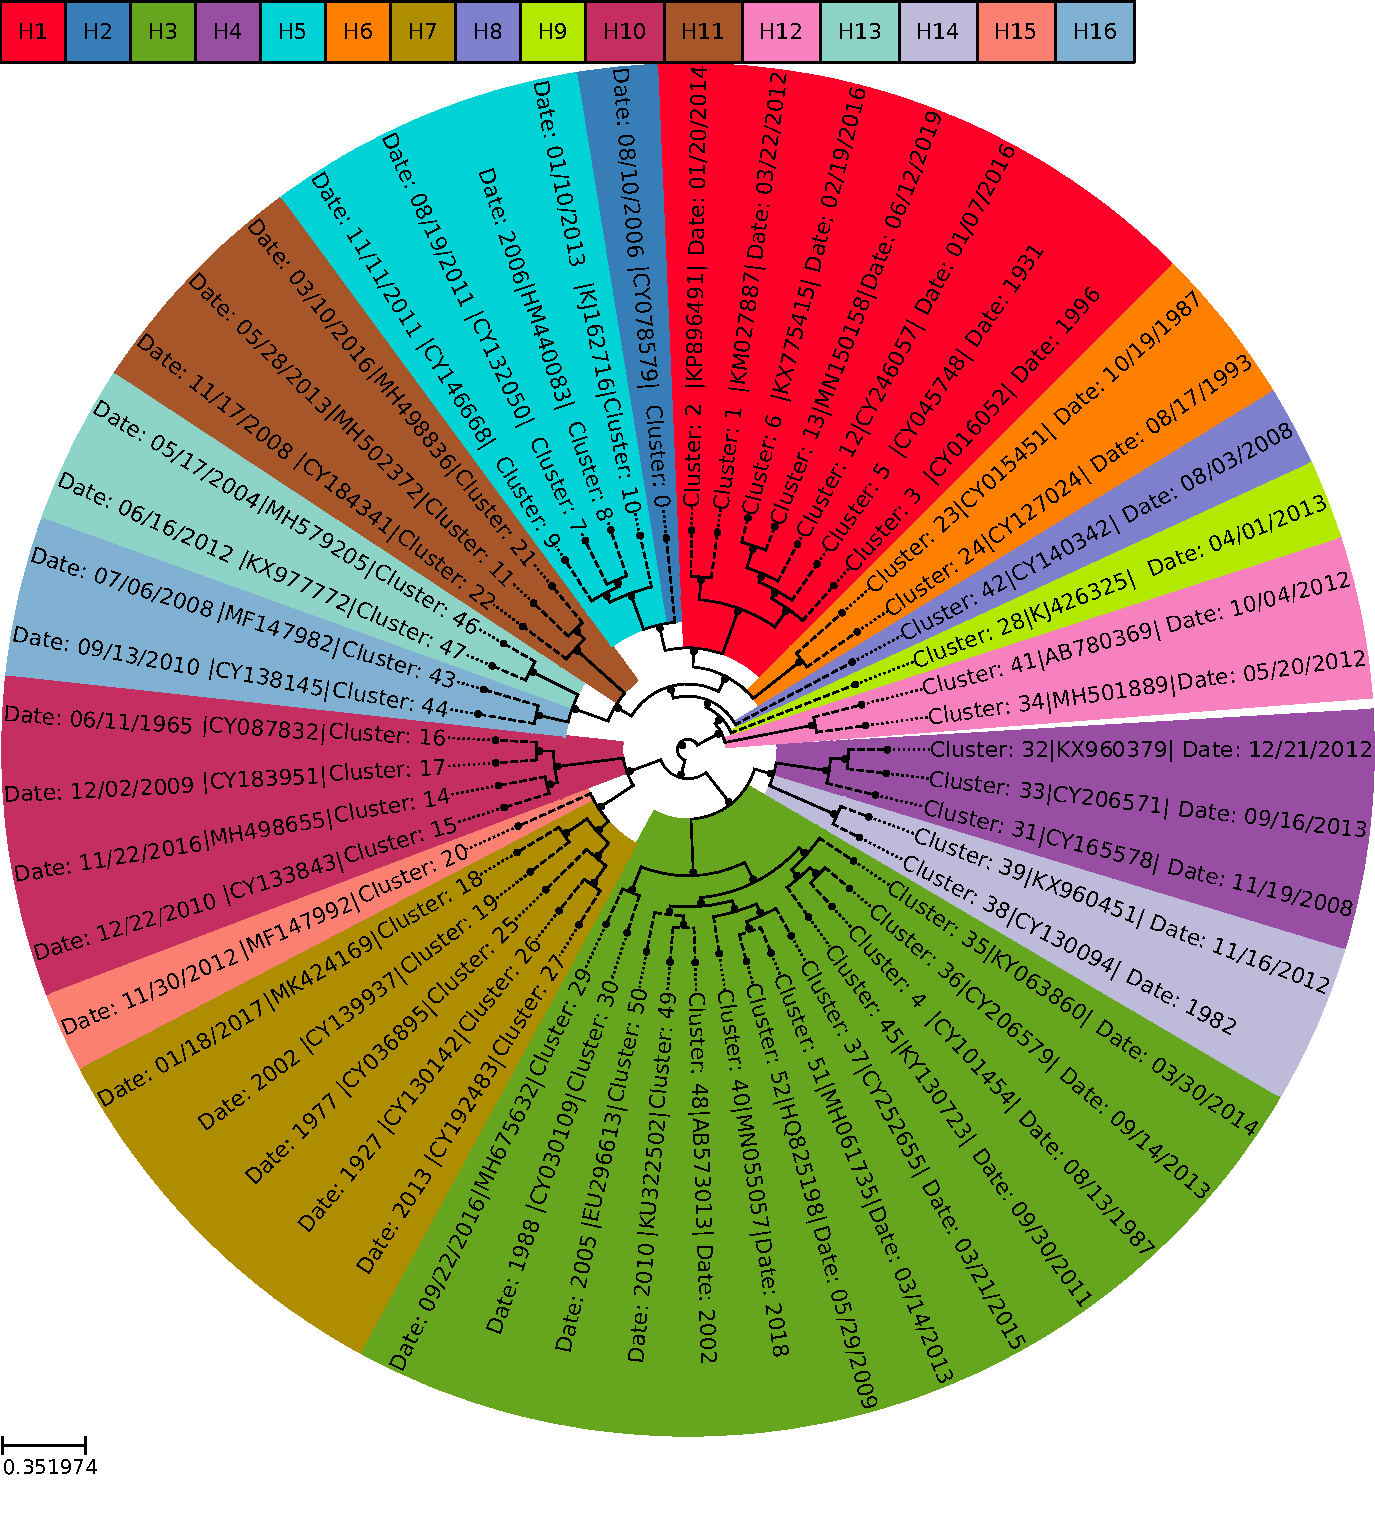
\includegraphics[width=\textwidth]{PCA/Guidetree_segment_4_H_Centroid.pdf}
    \caption[Knee based Segment 4 Centroid Guidetree (\texttt{PCA})]{\textbf{Knee based Segment 4 Centroid Guidetree (\texttt{PCA}).} The guide tree was created by building a \gls{MSA} on the centroid sequences of clusters resulting from the \texttt{PCA} and Kneedle Algorithm (PK) pipeline. The coloring of the tree is based on the related subtype of the centroid sequence used for the \gls{MSA}.}
    \label{fig:PCA_Guidetree_Centroid_4}
\end{figure}

Cluster 4 homogeneous for subtype H3 is split off the other H3 clusters by nearly all the non H3 clusters \autoref{fig:PCA_Cluster_Knee_4} \textbf{\textsf{D}}. By evaluation of the clusters relation with a guide-tree from the centroid sequences the error persists. Every of the 55 clusters have a sequence that should represent the whole cluster, the centroid sequence, calculated as described in \autoref{sec:MAFFT}. By building an alignment over these 55 centroid sequences a guide-tree was created (\autoref{fig:PCA_Guidetree_Centroid_4}). When using the guide-tree as comparison the uniform color distribution stood out. Even the mentioned cluster 4 is arranged in a line with all cluster homogeneous for subtype H3. The subset of the centroid sequences used for the guide tree might be to small for a sure proof but still the centroid sequences should be the most meaningful ones representing the whole cluster. Therefore cluster 4 and 48 (\autoref{fig:PCA_Cluster_Knee_4} \textbf{\textsf{C}} and \textbf{\textsf{D}}) remained as identified clustering mistakes and are further examined in the following.

%Übergang zu cluster Comparison durch Centroid Alignment Tree -> H13/H16 Clustertree, Alignmenttree Vergleich -> Cluster H13/H16 Comparison
%fehler im clustering oder fehler in der DAtenbank